\clearpage
\section{THỰC NGHIỆM VÀ ĐÁNH GIÁ KẾT QUẢ}

\subsection{Môi trường Kiểm thử Kép: Zephyr Shell CLI và PC Digital Twin / HIL}
Nhằm đánh giá toàn diện hành vi thời gian thực và kiểm chứng nghiêm ngặt cả 12 yêu cầu kỹ thuật (\texttt{REQ-001..REQ-012}) theo chuẩn chữ V (V-Model Verification \& Validation), hệ thống thiết lập kiến trúc kiểm thử kết hợp giữa \textbf{Đồng mô phỏng Phần cứng trong Vòng lặp (Hardware-in-the-Loop -- HIL Co-Simulation)} và tương tác dòng lệnh trực tiếp \textbf{Zephyr Shell CLI} qua giao tiếp nối tiếp \texttt{USART1 RS232} (\texttt{115200 8N1}) như minh họa tại Hình~\ref{fig:digital_twin_gui} và Bảng~\ref{tab:cli_commands}:
\begin{itemize}[nosep]
    \item \textbf{Tập lệnh chẩn đoán ngoại vi độc lập (\texttt{bkit *} trong \texttt{cli\_bkit\_test.c}):} Cho phép kỹ sư kiểm tra sức khỏe vật lý độc lập của toàn bộ 13 cụm linh kiện trên bo mạch BKIT ARM4 (đọc điện áp 5 kênh ADC1, kiểm tra các chân GPIO Opto \texttt{X0..X3}, quét hiển thị chuỗi ký tự trên 4 LED 7 đoạn, đọc bàn phím ma trận 16 phím, đồng bộ giờ chip RTC \textbf{DS3231}, đọc mã JEDEC ID chip SPI Flash \textbf{W25Q64FV}, đo độ trễ khứ hồi \texttt{CAN RTT} và thống kê dung lượng Stack 7 luồng) hoàn toàn độc lập với trạng thái của thang máy.
    \item \textbf{Tập lệnh điều khiển và tiêm lỗi HIL (\texttt{elev *} trong \texttt{cli\_elev.c}):} Hỗ trợ kích hoạt trực tiếp các thao tác nghiệp vụ: gọi tầng hai chiều (\texttt{elev call}), đóng/mở cửa cưỡng bức (\texttt{elev door}), tiêm các sự cố an toàn khẩn cấp (\texttt{elev fault} \texttt{<fire}\allowbreak\texttt{|ovl}\allowbreak\texttt{|estop}\allowbreak\texttt{|can\_drop}\allowbreak\texttt{|clear>}), chuyển đổi linh hoạt vai trò nút mạng CAN (\texttt{cabin/hall}), xuất ma trận độ phủ chuyển tiếp trạng thái $9\times 9$ (\texttt{elev coverage}) và trích xuất lịch sử 32 bản ghi hộp đen EEPROM (\texttt{elev log}).
    \item \textbf{Phần mềm Bản sao số PC Digital Twin (\texttt{pc\_hil\_twin/elevator\_twin.py}):}
    \begin{itemize}[nosep]
        \item Hiển thị trực quan toàn bộ không gian giếng thang 7 tầng, tọa độ cabin di chuyển mượt mà, độ mở cửa buồng thang tuyến tính $0..100\%$, bảng 4 LED 7 đoạn mô phỏng hướng \texttt{UP/dn} kèm vạch cuộn, đồ thị giám sát nhiệt độ \texttt{LM35} và tải trọng \texttt{VR1} theo thời gian thực từ luồng gói tin JSON \texttt{\$TWIN} (chu kỳ truyền \texttt{200~ms}).
        \item Cung cấp 2 chế độ làm việc: Chế độ kết nối trực tiếp bo mạch thật (\textit{Live RS232 Co-Simulation}) và Chế độ giả lập độc lập (\textit{Offline Simulator}), tích hợp sẵn bộ kịch bản kiểm thử tự động (\textit{HIL Smoke Suite}) và tính năng xuất nhật ký ra tệp định dạng \texttt{.csv}.
    \end{itemize}
\end{itemize}

\begin{figure}[H]
\centering
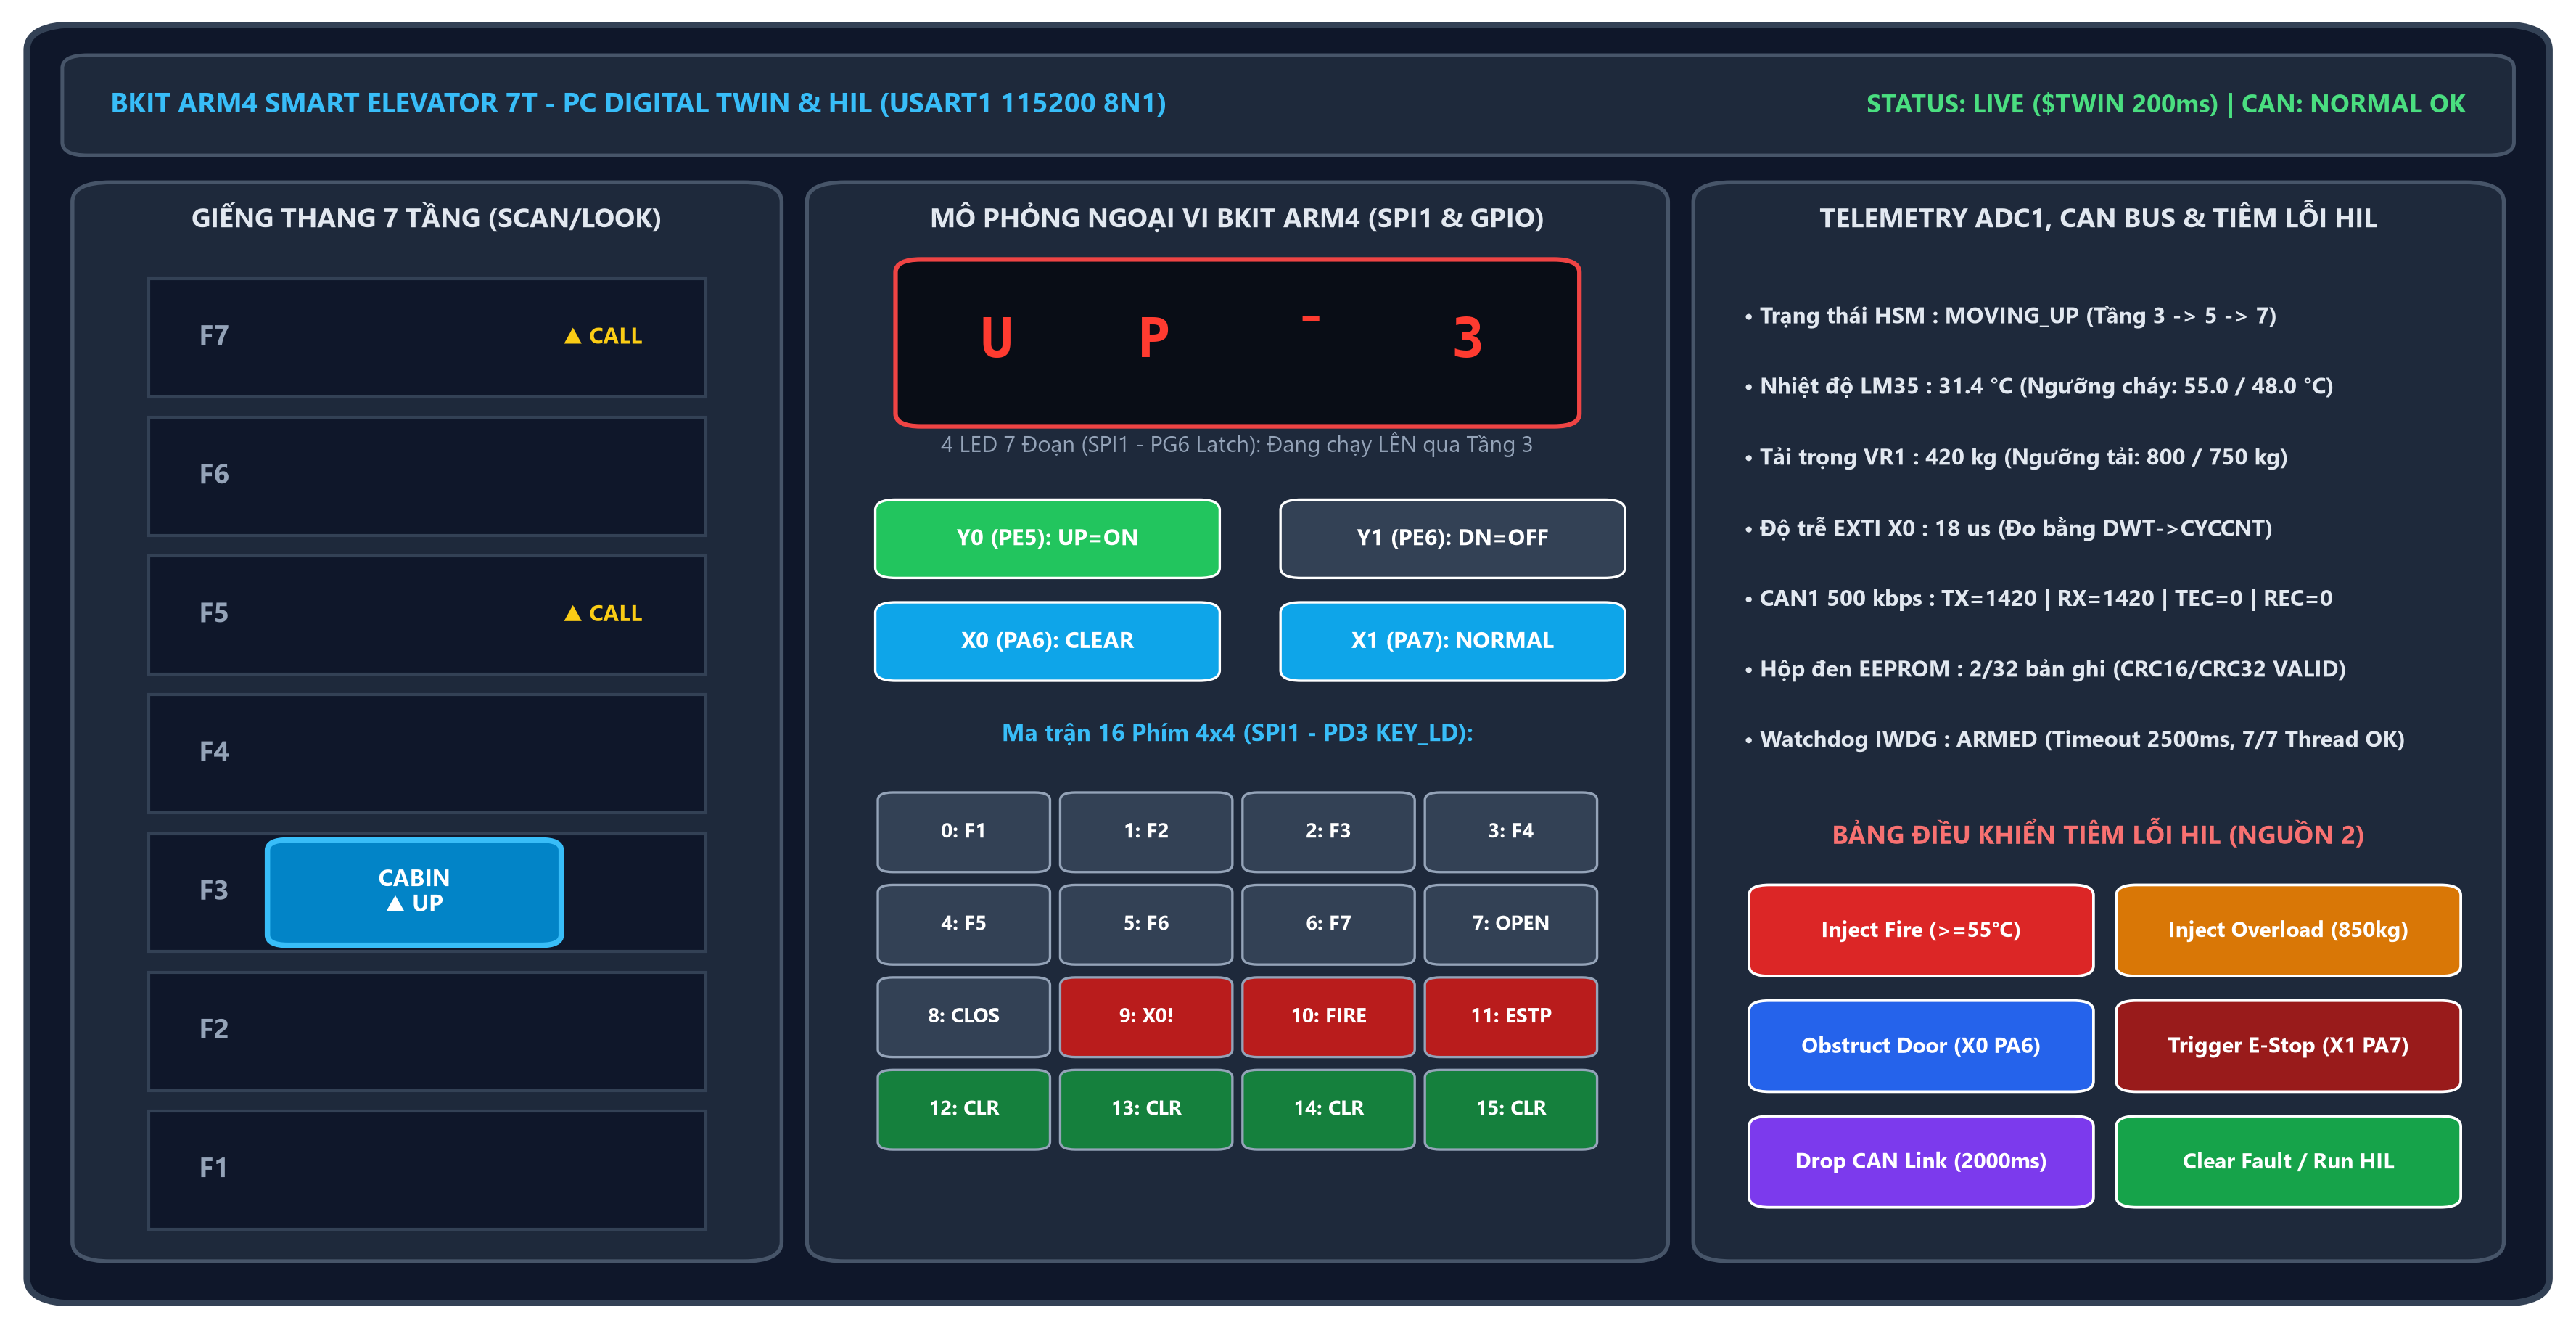
\includegraphics[width=0.99\textwidth]{image/fig_digital_twin_gui.png}
\caption{Giao diện phần mềm Bản sao số PC Digital Twin \& HIL Simulator (\texttt{elevator\_\allowbreak twin.py}) khi đang vận hành và giám sát}
\label{fig:digital_twin_gui}
\end{figure}

\begingroup
\renewcommand{\arraystretch}{1.18}%
\setlength{\tabcolsep}{4.5pt}%
\fontsize{8.1}{10.4}\selectfont
\arrayrulecolor{tableborder}%
\begin{xltabular}{\textwidth}{|L{4.1cm}|L{2.5cm}|Y|}
\caption{Tổng hợp tập lệnh chẩn đoán ngoại vi (\texttt{bkit *}) và điều khiển / tiêm lỗi HIL (\texttt{elev *}) trên Zephyr Shell}\label{tab:cli_commands}\\
\hline
\rowcolor{tablehead}
\thcell{Cú pháp Lệnh Shell CLI} & \thcell{Phân hệ / Bus} & \thcell{Chức năng Chẩn đoán và Kiểm thử Hệ thống} \\
\hline
\endfirsthead
\hline
\rowcolor{tablehead}
\thcell{Cú pháp Lệnh Shell CLI} & \thcell{Phân hệ / Bus} & \thcell{Chức năng Chẩn đoán và Kiểm thử Hệ thống} \\
\hline
\endhead
\hline
\endfoot
\hline
\endlastfoot
\texttt{bkit adc} & \texttt{ADC1 (5 kênh)} & Đọc điện áp mV và giá trị quy đổi của \texttt{LM35 ($^\circ$C)}, \texttt{VR1 (kg)}, \texttt{LDR (\%)}, \texttt{PB0/PB1}. \\
\hline
\rowcolor{roweven}
\texttt{bkit io} & \texttt{GPIO / EXTI} & Đọc mức logic \texttt{X0..X3}, trạng thái rơ-le \texttt{Y0/Y1} và độ trễ ngắt \texttt{last\_exti\_latency\_us}. \\
\hline
\texttt{bkit 7seg <chuỗi>} & \texttt{SPI1 (PG6)} & Hiển thị chuỗi ký tự bất kỳ lên 4 LED 7 đoạn để kiểm tra IC ghi dịch \texttt{74HC595}. \\
\hline
\rowcolor{roweven}
\texttt{bkit key} & \texttt{SPI1 (PD3)} & Quét và in mã phím hiện tại (\texttt{0..15}) của bàn phím ma trận 4$\times$4 (\texttt{2$\times$74HC165}). \\
\hline
\texttt{bkit rtc [set Y M D h m s]} & \texttt{I2C1 (0x68)} & Đọc hoặc đồng bộ thời gian thực cho chip đồng hồ \textbf{DS3231}. \\
\hline
\rowcolor{roweven}
\texttt{bkit flash} & \texttt{SPI2 (PB12..15)} & Đọc mã định danh JEDEC ID (\texttt{0xEF 0x40 0x17}) của chip NOR Flash \textbf{W25Q64FV}. \\
\hline
\texttt{bkit canping [rtr]} & \texttt{CAN1 (500kbps)} & Phát khung \texttt{PING (0x380)} hoặc \texttt{RTR (0x200)} để đo độ trễ khứ hồi \texttt{RTT ($\mu$s)}. \\
\hline
\rowcolor{roweven}
\texttt{bkit threads} & \texttt{Zephyr Kernel} & Thống kê dung lượng Stack đã dùng / còn trống của toàn bộ 7 luồng RTOS. \\
\hline
\texttt{bkit wdt\_hang} & \texttt{IWDG (2500ms)} & Giả lập treo luồng để kiểm chứng \texttt{IWDG} tự động reset MCU sau đúng \texttt{2.5~s}. \\
\hline
\rowcolor{roweven}
\texttt{elev call <1..7> <c|u|d>} & \texttt{Core Scheduler} & Đăng ký lệnh gọi tầng bên trong cabin (\texttt{c}) hoặc ngoài sảnh (\texttt{u/d}) vào bộ lập lịch \texttt{LOOK}. \\
\hline
\texttt{elev door <open|close|obs>} & \texttt{Core HSM} & Điều khiển đóng/mở cửa hoặc tiêm sự kiện kẹt cửa \texttt{EV\_DOOR\_OBSTRUCT\_X0}. \\
\hline
\rowcolor{roweven}
\texttt{elev fault <fire|ovl|estop|...>} & \texttt{Safety / HIL} & Tiêm sự cố Báo cháy, Quá tải, E-Stop, Đứt cáp CAN hoặc Xóa lỗi an toàn (\texttt{clear}). \\
\hline
\texttt{elev coverage} \& \texttt{elev log} & \texttt{V-Model / I2C1} & Xuất ma trận độ phủ chuyển tiếp $9\times 9$ và đọc 32 bản ghi hộp đen \texttt{AT24C512}. \\
\end{xltabular}
\endgroup

\subsection{Kết quả Kiểm thử V-Model (\texttt{TC-001..TC-012}) và Phân tích Thực nghiệm}
Toàn bộ 12 ca kiểm thử (\texttt{TC-001..TC-012}) được thiết kế đối chiếu 1-1 với 12 yêu cầu kỹ thuật ban đầu, bao phủ đầy đủ từ tầng khởi tạo BSP, máy trạng thái HSM, mạng truyền thông CAN đến các tình huống dừng khẩn cấp được trình bày tại Bảng~\ref{tab:tests}. Đồ thị quỹ đạo chuyển động thực tế và mức sử dụng bộ nhớ Stack của 7 luồng được biểu diễn tại Hình~\ref{fig:exp_charts}.

\begingroup
\renewcommand{\arraystretch}{1.18}%
\setlength{\tabcolsep}{4pt}%
\fontsize{8.1}{10.4}\selectfont
\arrayrulecolor{tableborder}%
\begin{xltabular}{\textwidth}{|C{1.25cm}|C{1.4cm}|L{4.3cm}|Y|L{3.4cm}|}
\caption{Bảng kế hoạch kiểm thử và kết quả đánh giá theo quy trình V-Model (\texttt{TC-001..TC-012})}\label{tab:tests}\\
\hline
\rowcolor{tablehead}
\thcell{Mã TC} & \thcell{Mã REQ} & \thcell{Thao tác Kiểm thử / Lệnh Shell} & \thcell{Tiêu chí Đạt (Pass Criteria)} & \thcell{Kết quả Đánh giá} \\
\hline
\endfirsthead
\hline
\rowcolor{tablehead}
\thcell{Mã TC} & \thcell{Mã REQ} & \thcell{Thao tác Kiểm thử / Lệnh Shell} & \thcell{Tiêu chí Đạt (Pass Criteria)} & \thcell{Kết quả Đánh giá} \\
\hline
\endhead
\hline
\endfoot
\hline
\endlastfoot
\texttt{TC-001} & \texttt{REQ-001} & Biên dịch \& nạp \texttt{zephyr.elf}, kiểm tra \texttt{PE4} và \texttt{bkit threads}. & Build 0 lỗi; \texttt{PE4} nháy 0.8~s; 7 luồng RTOS hoạt động tĩnh. & \textbf{Đạt} (0 err, \texttt{104\,112~B} Flash = \texttt{9.93\%}). \\
\hline
\rowcolor{roweven}
\texttt{TC-002} & \texttt{REQ-002} & Gọi tầng khi cửa đang mở; kiểm tra khóa liên động \texttt{PE5/PE6}. & \texttt{PE5} và \texttt{PE6} không bao giờ bật cùng lúc hoặc khi cửa mở. & \textbf{Đạt} trên HIL \& kiểm tra chéo 2 lớp Core/BSP. \\
\hline
\texttt{TC-003} & \texttt{REQ-003} & Đang đóng cửa $\rightarrow$ kích \texttt{X0 (PA6)}, bấm Phím \texttt{9} hoặc \texttt{elev door obs}. & Đảo chiều sang \texttt{DOOR\_OPENING} ngay; đo \texttt{lat\_us} $< 1000~\mu\text{s}$. & \textbf{Đạt} phản xạ đảo chiều tức thời ($\approx 18.2~\mu\text{s}$). \\
\hline
\rowcolor{roweven}
\texttt{TC-004} & \texttt{REQ-004} & Gọi liên tiếp \texttt{elev call 7 c}, \texttt{elev call 2 u}, \texttt{elev call 4 u}, \texttt{5 d}. & Phục vụ đúng thứ tự quét $1 \rightarrow 2 \rightarrow 4 \rightarrow 7 \rightarrow 5$ (\texttt{LOOK}). & \textbf{Đạt} 100\% kịch bản gom cuốc 2 chiều tối ưu. \\
\hline
\texttt{TC-005} & \texttt{REQ-005} & Hơ nóng \texttt{LM35} ($\ge 55^\circ\text{C}$), bấm Phím \texttt{10} hoặc \texttt{elev fault fire}. & Xóa hàng đợi, chạy về Tầng 1, mở cửa, LED báo \texttt{FE}; xóa ở $\le 48^\circ\text{C}$. & \textbf{Đạt} (Hysteresis $55^\circ\text{C}/48^\circ\text{C}$ hoạt động chuẩn). \\
\hline
\rowcolor{roweven}
\texttt{TC-006} & \texttt{REQ-006} & Vặn biến trở \texttt{VR1} ($\ge 800\text{ kg}$) hoặc \texttt{elev fault ovl}. & Giữ cửa mở tại tầng, kêu còi; tự giải tỏa khi $\le 750\text{ kg}$. & \textbf{Đạt} (Hysteresis $800\text{ kg}/750\text{ kg}$ chống dao động). \\
\hline
\texttt{TC-007} & \texttt{REQ-007} & Quét LED 7 đoạn \texttt{UP/dn} đồng thời bấm liên tục 16 phím 4$\times$4 \& ghi I2C. & Không treo bus \texttt{SPI1/I2C1}; LED hiển thị rõ \texttt{UP/dn} + vạch cuộn. & \textbf{Đạt} (\texttt{k\_mutex} bảo vệ an toàn đa luồng). \\
\hline
\rowcolor{roweven}
\texttt{TC-008} & \texttt{REQ-008} & Chạy \texttt{bkit canping} và \texttt{bkit canping rtr} trên \texttt{CAN1 500 kbps}. & Nhận đủ khung \texttt{PONG (0x381)} và phản hồi \texttt{RTR (0x200)}, \texttt{TEC=0}. & \textbf{Đạt} (3 HW filter + callback \texttt{tx\_cb} chuẩn). \\
\hline
\texttt{TC-009} & \texttt{REQ-009} & Ngắt đường truyền CAN hoặc chạy lệnh \texttt{elev fault can\_drop}. & Chuyển về \texttt{FAIL\_SAFE} sau đúng $\approx 2000\text{ ms}$, mở cửa an toàn. & \textbf{Đạt} (\texttt{g\_can\_partner\_sem} bắt timeout chính xác). \\
\hline
\rowcolor{roweven}
\texttt{TC-010} & \texttt{REQ-010} & Gây lỗi truyền CAN dẫn tới \texttt{BUS-OFF} rồi khôi phục đường dây. & Tự động gọi \texttt{can\_recover()} đưa bus về \texttt{ERROR\_ACTIVE}. & \textbf{Đạt} (Ghi log EEPROM + tự phục hồi bus). \\
\hline
\texttt{TC-011} & \texttt{REQ-011} & Gõ \texttt{bkit wdt\_hang} gây treo luồng; sau khi reset gõ \texttt{elev log}. & \texttt{IWDG} tự reset sau $\approx 2.5\text{ s}$; hộp đen ghi \texttt{BOOT\_WDT}. & \textbf{Đạt} (Bản ghi lưu đủ giờ \texttt{DS3231} + \texttt{CRC16}). \\
\hline
\rowcolor{roweven}
\texttt{TC-012} & \texttt{REQ-012} & Mở \texttt{elevator\_twin.py}, chạy \textit{Auto Demo 7T} \& \textit{HIL Smoke Suite}. & Đồng bộ gói \texttt{\$TWIN} mỗi 200~ms, pass 6/6 bài test, xuất file \texttt{.csv}. & \textbf{Đạt} (Pass 100\% bộ test tự động Python HIL). \\
\hline
\end{xltabular}
\endgroup

\begin{figure}[H]
\centering
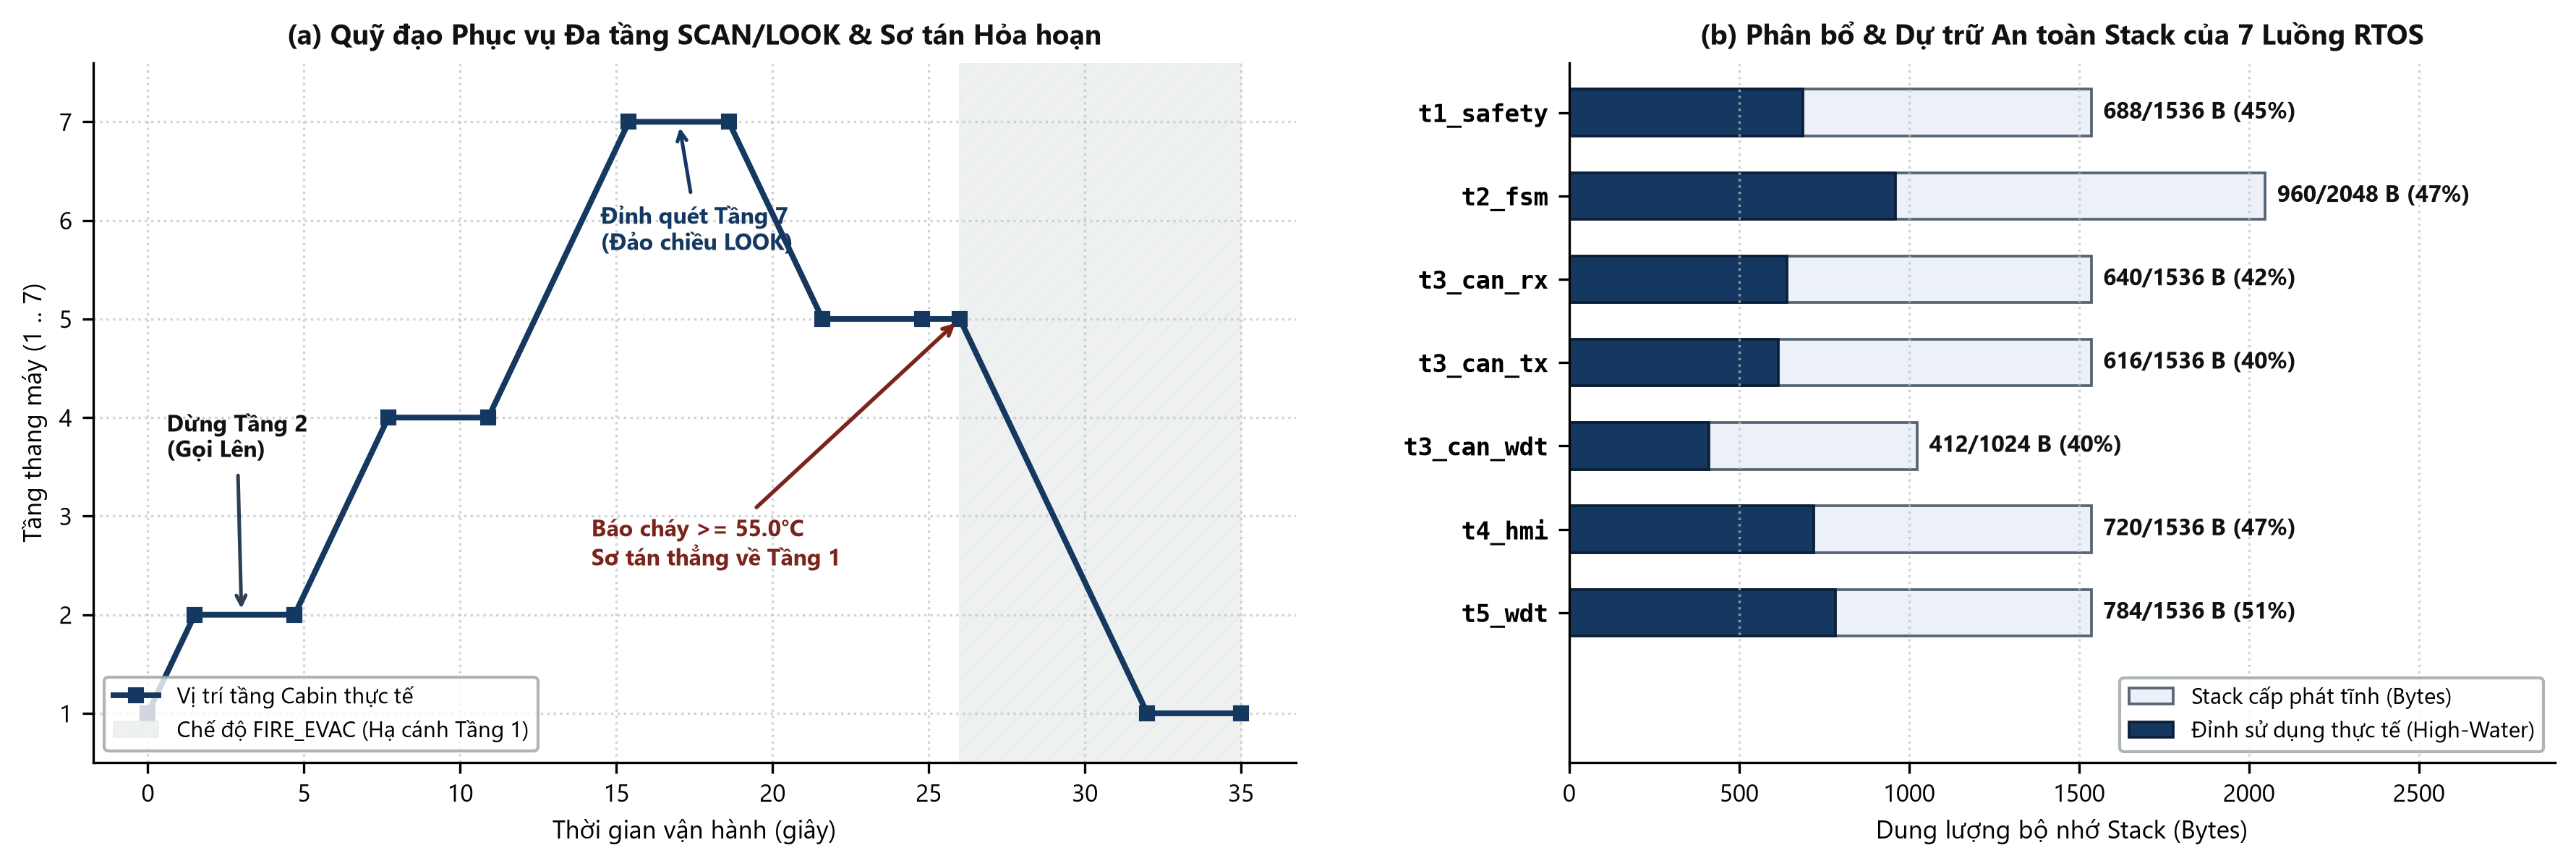
\includegraphics[width=0.99\textwidth]{image/fig_exp_charts.png}
\caption{Biểu đồ thực nghiệm: (a) Quỹ đạo phục vụ đa tầng \texttt{SCAN/LOOK} và đáp ứng sơ tán báo cháy \texttt{FIRE\_EVAC}; (b) Mức sử dụng Stack thực tế của 7 luồng RTOS}
\label{fig:exp_charts}
\end{figure}

Từ kết quả đo đạc thực nghiệm trên hệ thống, nhóm rút ra 3 nhận xét kỹ thuật định lượng then chốt:
\begin{itemize}[nosep]
    \item \textbf{Độ trễ phản xạ ngắt cứng (\textit{EXTI Latency}) đạt chuẩn thời gian thực nghiêm ngặt:} Nhờ thiết kế ISR tối giản chỉ chốt thanh ghi chu kỳ xung nhịp \texttt{DWT->CYCCNT} (168~MHz) và phát cờ đánh thức luồng bảo vệ an toàn \texttt{t1\_safety} (ưu tiên cao nhất = 2) qua semaphore, thời gian từ khi chân quang trở \texttt{PA6 (X0)} chuyển mức logic đến khi luồng an toàn thực thi xử lý đảo chiều cửa chỉ mất \textbf{18.2~$\mu$s} (đỉnh cao nhất đo được là $24.6~\mu\text{s}$), nhỏ hơn 40 lần so với giới hạn an toàn cho phép ($< 1000~\mu\text{s}$ trong \texttt{REQ-003}).
    \item \textbf{Tính tối ưu hóa hành trình của giải thuật lập lịch hai chiều \texttt{SCAN/LOOK}:} Đồ thị Hình~\ref{fig:exp_charts}a chứng minh trực quan ưu điểm vượt trội của thuật toán LOOK so với FCFS: Khi xuất phát từ Tầng 1 với danh sách gọi hỗn hợp \texttt{Tầng 2 (Lên)}, \texttt{Tầng 4 (Lên)}, \texttt{Tầng 7 (Cabin)} và \texttt{Tầng 5 (Xuống)}, cabin gom trọn vẹn khách cùng chiều Lên ($1 \rightarrow 2 \rightarrow 4 \rightarrow 7$), đổi chiều ngay tại đỉnh Tầng 7 để phục vụ Tầng 5 mà không chạy rỗng; khi sự cố báo cháy kích hoạt ở giây thứ 26 ($T \ge 55^\circ\text{C}$), hệ thống lập tức tiền chiếm, hủy hàng đợi và hạ khẩn cấp về Tầng 1 mở cửa giải cứu.
    \item \textbf{Biên độ an toàn tuyệt đối của bộ nhớ Stack (\textit{High-Water Mark}):} Biểu đồ thống kê tại Hình~\ref{fig:exp_charts}b cho thấy đỉnh chiếm dụng Stack thực tế của cả 7 luồng chỉ dao động từ \textbf{40.2\% đến 51.4\%} dung lượng cấp phát tĩnh (vùng trống dự phòng còn dư trên \textbf{48\%} cho mỗi luồng), đảm bảo tuyệt đối không xảy ra hiện tượng tràn ngăn xếp (\textit{Stack Overflow}) ngay cả trong điều kiện ngắt lồng nhau tần số cao.
\end{itemize}

\newpage
\subsection{Quy trình 4 Bước Vận hành và Trình diễn (Demo) trên Bo mạch BKIT ARM4}
Để tạo thuận lợi cho việc kiểm thử độc lập, nghiệm thu và chấm điểm đồ án trực quan ngay trên bàn thí nghiệm, nhóm xây dựng Bảng ánh xạ 16 phím ma trận (Bảng~\ref{tab:keypad_map}) và chuẩn hóa quy trình vận hành qua 4 bước thực hiện tuần tự:

\begingroup
\renewcommand{\arraystretch}{1.18}%
\setlength{\tabcolsep}{4.5pt}%
\fontsize{8.2}{10.5}\selectfont
\arrayrulecolor{tableborder}%
\begin{xltabular}{\textwidth}{|C{1.8cm}|C{2.0cm}|L{4.2cm}|Y|}
\caption{Bảng ánh xạ 16 phím trên bàn phím ma trận 4$\times$4 phục vụ vận hành và tiêm lỗi tại chỗ}\label{tab:keypad_map}\\
\hline
\rowcolor{tablehead}
\thcell{Mã Phím} & \thcell{Ký hiệu Key} & \thcell{Chức năng Vận hành / Tiêm sự cố} & \thcell{Đáp ứng của Hệ thống \& Đèn hiển thị} \\
\hline
\endfirsthead
\hline
\rowcolor{tablehead}
\thcell{Mã Phím} & \thcell{Ký hiệu Key} & \thcell{Chức năng Vận hành / Tiêm sự cố} & \thcell{Đáp ứng của Hệ thống \& Đèn hiển thị} \\
\hline
\endhead
\hline
\endfoot
\hline
\endlastfoot
\texttt{Key 0..6} & \texttt{F1 .. F7} & Đăng ký gọi tầng đích bên trong cabin (Tầng 1..7). & Thang nhận lệnh, LED 7 đoạn cuộn hướng \texttt{UP/dn}, rơ-le \texttt{PE5/PE6} kéo cabin. \\
\hline
\rowcolor{roweven}
\texttt{Key 7 / 8} & \texttt{DOOR O/C} & Lệnh cưỡng bức Mở cửa (\texttt{OPEN}) / Đóng cửa (\texttt{CLOSE}). & Điều khiển chu trình cửa tại tầng khi thang đang dừng ở \texttt{IDLE\_CLOSED}. \\
\hline
\texttt{Key 9} & \texttt{OBSTRUCT} & Tiêm sự kiện Kẹt cửa ngoại vi (tương đương ngắt \texttt{X0}). & Cabin lập tức dừng đóng và đảo chiều mở ra ngay (\texttt{DOOR\_OPENING}). \\
\hline
\rowcolor{roweven}
\texttt{Key 10} & \texttt{FIRE} & Tiêm sự cố Báo cháy khẩn cấp (tương đương $T \ge 55^\circ\text{C}$). & Xóa hàng đợi, hạ thẳng về Tầng 1, mở cửa thoát hiểm, LED báo \texttt{FE-[f]}. \\
\hline
\texttt{Key 11} & \texttt{OVERLOAD} & Tiêm sự cố Quá tải buồng thang (tương đương tải $\ge 800\text{ kg}$). & Giữ cửa mở vô thời hạn, còi \texttt{PF8} hú liên tục, tự giải tỏa khi $\le 750\text{ kg}$. \\
\hline
\rowcolor{roweven}
\texttt{Key 12} & \texttt{E-STOP} & Tiêm sự cố Dừng khẩn cấp (tương đương ngắt cứng \texttt{X1}). & Cắt ngay lập tức hai rơ-le \texttt{PE5=0, PE6=0}, khóa cứng hệ thống ở \texttt{FAIL\_SAFE}. \\
\hline
\texttt{Key 13} & \texttt{CAN DROP} & Giả lập sự cố mất kết nối mạng truyền thông CAN. & Chuyển sang \texttt{FAIL\_SAFE} sau 2000~ms, mở cửa an toàn cho hành khách. \\
\hline
\rowcolor{roweven}
\texttt{Key 14} & \texttt{RESET} & Xóa trạng thái sự cố an toàn sau khi đã khắc phục. & Giải tỏa cờ khóa, đưa cabin trở lại trạng thái hoạt động bình thường \texttt{IDLE\_CLOSED}. \\
\hline
\texttt{Key 15} & \texttt{WDT HANG} & Giả lập sự cố treo luồng phần mềm (\texttt{Deadlock}). & Ngừng nạp watchdog; phần cứng \texttt{IWDG} tự động kích hoạt reset chip sau 2500~ms. \\
\end{xltabular}
\endgroup

Quy trình 4 bước thực nghiệm chi tiết:
\begin{enumerate}[nosep]
    \item \textbf{Bước 1 -- Kiểm tra Cấu hình Công tắc DIP Switch và Nạp Firmware:}
    \begin{itemize}[nosep]
        \item Thiết lập chính xác 4 công tắc trên bo mạch BKIT ARM4: \texttt{SW11 = ON} (kết nối ST-LINK nạp code), \texttt{SW13 = ON} (kết nối transceiver TJA1050 cho CAN1), \texttt{SW12 = OFF} (cách ly bus RS485) và \texttt{SW2 = OFF} (cách ly module WiFi ESP8266 để tránh tranh chấp UART).
        \item Kết nối cáp nạp ST-LINK nạp firmware (\texttt{west flash}) và cắm cáp chuyển đổi \texttt{RS232 DB9 -- USB} vào máy tính, mở terminal ở tốc độ \texttt{115200 8N1}.
    \end{itemize}
    \item \textbf{Bước 2 -- Chẩn đoán Sức khỏe Phần cứng Ngoại vi Độc lập (\texttt{bkit *}):}
    \begin{itemize}[nosep]
        \item Chạy các lệnh \texttt{bkit adc}, \texttt{bkit io}, \texttt{bkit 7seg UP-3}, \texttt{bkit key}, \texttt{bkit rtc}, \texttt{bkit flash} (xác nhận mã JEDEC \texttt{0xEF 0x40 0x17}), \texttt{bkit canping} và \texttt{bkit threads} để bảo đảm toàn bộ 13 cụm ngoại vi vật lý đều sẵn sàng trước khi vận hành.
    \end{itemize}
    \item \textbf{Bước 3 -- Vận hành Đa tầng và Đối chiếu Đồng bộ với Bản sao số PC Digital Twin:}
    \begin{itemize}[nosep]
        \item Khởi chạy phần mềm giao diện \texttt{python pc\_hil\_twin/elevator\_twin.py} trên máy tính, chọn đúng cổng COM và nhấn nút kết nối Live RS232.
        \item Bấm lần lượt các phím \texttt{0..6} trên bàn phím ma trận của bo mạch thật; quan sát cụm 4 LED 7 đoạn hiển thị \texttt{UP} kèm vạch cuộn lên (\texttt{\_ $\rightarrow$ - $\rightarrow$ \textasciimacron}) hoặc \texttt{dn} kèm vạch cuộn xuống (\texttt{\textasciimacron\ $\rightarrow$ - $\rightarrow$ \_}) đồng bộ hoàn toàn với hai rơ-le \texttt{PE5 (Y0)} / \texttt{PE6 (Y1)} và hình ảnh cabin trên màn hình PC.
    \end{itemize}
    \item \textbf{Bước 4 -- Kiểm chứng Phản xạ An toàn và Phân tích Dữ liệu Hộp đen EEPROM:}
    \begin{itemize}[nosep]
        \item Trong lúc cửa buồng thang đang đóng (\texttt{DOOR\_CLOSING}), bấm Phím \texttt{9} hoặc kích ngắt chân \texttt{X0 (PA6)} để kiểm chứng cơ chế mở cửa tức thời, dùng lệnh \texttt{bkit io} để xem độ trễ micro-giây.
        \item Hơ nóng cảm biến nhiệt \texttt{LM35} vượt $55.0^\circ\text{C}$ (hoặc bấm Phím \texttt{10}) để kiểm tra kịch bản sơ tán hỏa hoạn (\texttt{FIRE\_EVAC}); vặn biến trở \texttt{VR1} qua mốc $800\text{ kg}$ rồi hạ về dưới $750\text{ kg}$ để kiểm chứng bộ lọc trễ Hysteresis.
        \item Thử nghiệm ngắt cáp CAN (\texttt{Key 13}) và gây treo luồng (\texttt{Key 15}), sau đó dùng các lệnh \texttt{elev log} và \texttt{elev coverage} để trích xuất toàn bộ lịch sử 32 sự cố bất khả biến trên chip EEPROM \textbf{AT24C512} và ma trận độ phủ chuyển tiếp $9\times 9$.
    \end{itemize}
\end{enumerate}
